\chaptertitlepage{Methodology}

This chapter describes how we built and evaluated the system. Besides classifying chest X-rays, the methodology had to let us compare three deep learning architectures fairly and reproducibly, so all three are trained under the same conditions. The pipeline has six stages: merging the datasets, preprocessing and augmentation, model design, training, evaluation with a leakage check, and deployment in Flask with ensemble inference.

\begin{figure}[H]
\centering
\begin{tikzpicture}[
  node distance=0.45cm and 0.35cm,
  every node/.style={font=\footnotesize\sffamily}
]
\node[diag start, minimum width=2.1cm] (s1) {Public CXR\\sources};
\node[diag step, right=of s1, minimum width=2.1cm] (s2) {Build unified\\manifest};
\node[diag step, right=of s2, minimum width=2.1cm] (s3) {Preprocess +\\augment};
\node[diag step, right=of s3, minimum width=2.1cm] (s4) {Train three\\architectures};
\node[diag step, below=1.1cm of s4, minimum width=2.1cm] (s5) {Evaluate +\\leakage probe};
\node[diag out, left=of s5, minimum width=2.1cm] (s6) {Flask ensemble\\deployment};

\draw[diag arrow] (s1) -- (s2);
\draw[diag arrow] (s2) -- (s3);
\draw[diag arrow] (s3) -- (s4);
\draw[diag arrow] (s4) -- (s5);
\draw[diag arrow] (s5) -- (s6);

\node[diag label, below=0.15cm of s2] {dedupe, patient splits};
\node[diag label, below=0.15cm of s3] {model-specific sizes};
\node[diag label, below=0.15cm of s6] {soft voting + X-ray gate};
\end{tikzpicture}
\caption{End-to-end methodology pipeline for the unified four-class system}
\label{fig:method-pipeline}
\end{figure}

\section{From Single-Disease Models to a Unified Benchmark}

The first version of this project used three separate models with incompatible label sets: binary tuberculosis, multi-class COVID-19 screening (which at the time included Viral Pneumonia), and binary pneumonia. We could not compare them properly, since a difference in performance might come from the datasets and say nothing about the architectures. We therefore reframed the problem as a single four-class task and trained all three architectures on the same merged dataset, with the same patient-grouped splits, the same classification head for the transfer models, and the same training budget. The class order is fixed as Normal, Tuberculosis, COVID-19, Pneumonia. Images labelled Viral Pneumonia in the COVID sources are counted as Pneumonia, because the Kaggle pneumonia dataset mixes bacterial and viral cases and there is no way to separate them after the fact.

\section{Data Collection and Unified Manifest}

We did not collect any new clinical data. A builder script (\path{training/build_manifest.py}) merges three public datasets into \path{training/manifest.csv}, which records each image's path, class, patient identifier, source dataset, and split (train, validation, or test).

\subsection{Source Datasets}

\begin{table}[H]
\centering
\caption{Source datasets used to construct the unified four-class corpus}
\label{tab:method-datasets}
\small
\begin{adjustbox}{max width=\textwidth}
\begin{tabular}{@{}P{3.4cm}P{4.0cm}P{4.2cm}@{}}
\toprule
\HeaderRow \Head{Source dataset} & \Head{Expected path} & \Head{Classes contributed} \\
\midrule
TB Chest X-Ray (Kaggle) & \path{TB_Chest_Radiography_Database/} & Tuberculosis, Normal \\
\ZebraRow Covid19-dataset & \path{DenseNet121/Covid19-dataset/} & COVID-19, Normal, Pneumonia \\
Chest X-Ray Pneumonia (Kaggle) & \path{pneumonia_detection/data/chest_xray/} & Pneumonia, Normal \\
\bottomrule
\end{tabular}
\end{adjustbox}
\end{table}

\begin{figure}[H]
\centering
\begin{tikzpicture}[node distance=0.55cm and 0.55cm]
\node[diag step, minimum width=2.6cm] (tb) {TB CXR\\database};
\node[diag step, below=of tb, minimum width=2.6cm] (cov) {COVID-19\\dataset};
\node[diag step, below=of cov, minimum width=2.6cm] (pn) {Pneumonia\\CXR dataset};

\node[diag start, right=1.4cm of cov, minimum width=2.8cm] (merge) {Merge +\\hash dedupe};
\node[diag step, right=of merge, minimum width=2.6cm] (split) {Patient-grouped\\train/val/test};
\node[diag out, right=of split, minimum width=2.4cm] (man) {manifest.csv\\4 classes};

\draw[diag arrow] (tb.east) -- ++(0.55,0) |- (merge.west);
\draw[diag arrow] (cov) -- (merge);
\draw[diag arrow] (pn.east) -- ++(0.55,0) |- (merge.west);
\draw[diag arrow] (merge) -- (split);
\draw[diag arrow] (split) -- (man);

\node[diag label, below=0.12cm of man] {Normal $\cdot$ TB $\cdot$ COVID-19 $\cdot$ Pneumonia};
\end{tikzpicture}
\caption{Dataset unification into a shared four-class training manifest}
\label{fig:data-unify}
\end{figure}

\subsection{Design Rules for Honest Splits}

Six rules keep the splits honest:

\begin{enumerate}
    \item \textbf{Content-hash deduplication.} We remove byte-identical images, so the same file cannot end up in both the training and test sets.
    \item \textbf{Patient-grouped splitting.} All images from one patient go into the same split, whether that is train, validation, or test.
    \item \textbf{Fully qualified patient IDs.} Bare file names such as \texttt{0101.jpeg} repeat across the COVID folders, so we qualify each identifier with its path and group patients across the whole dataset.
    \item \textbf{Multi-source Normal and Pneumonia.} Both classes draw on more than one dataset, which makes it harder for a model to tell classes apart by scanner or dataset style.
    \item \textbf{Class-size capping with class weights.} COVID-19 has only $130$ images after deduplication. We capped the other classes at 1{,}200 in the reported run (\texttt{--cap 1200}) and handled the remaining imbalance with inverse-frequency class weights (COVID-19 weight $\approx$ 2.851).
    \item \textbf{Class$\times$source inspection.} Before training, we check a class-by-source table to confirm that Normal and Pneumonia really do come from several datasets.
\end{enumerate}

Every image comes from a public research dataset. The system is a research demonstration and a benchmark of architectures; it has not been clinically validated and is not a diagnostic device.

\section{Preprocessing and Data Augmentation}

\subsection{Model-Specific Preprocessing}

\begin{table}[H]
\centering
\caption{Preprocessing per architecture}
\label{tab:method-preprocess}
\small
\begin{tabular}{@{}llc@{}}
\toprule
\HeaderRow \Head{Model} & \Head{Input size} & \Head{Preprocessing} \\
\midrule
EfficientNetB3 & $256\times256\times3$ & EfficientNet \texttt{preprocess\_input} \\
\ZebraRow DenseNet121 & $224\times224\times3$ & DenseNet \texttt{preprocess\_input} \\
Custom CNN & $150\times150\times3$ & Divide by 255 \\
\bottomrule
\end{tabular}
\end{table}

Training and inference decode and resize images the same way, with bilinear interpolation. An earlier version resized with nearest-neighbour at inference but bilinear during training. That mismatch (train--serve skew) changed a large fraction of pixel values, so we fixed it.

\begin{figure}[H]
\centering
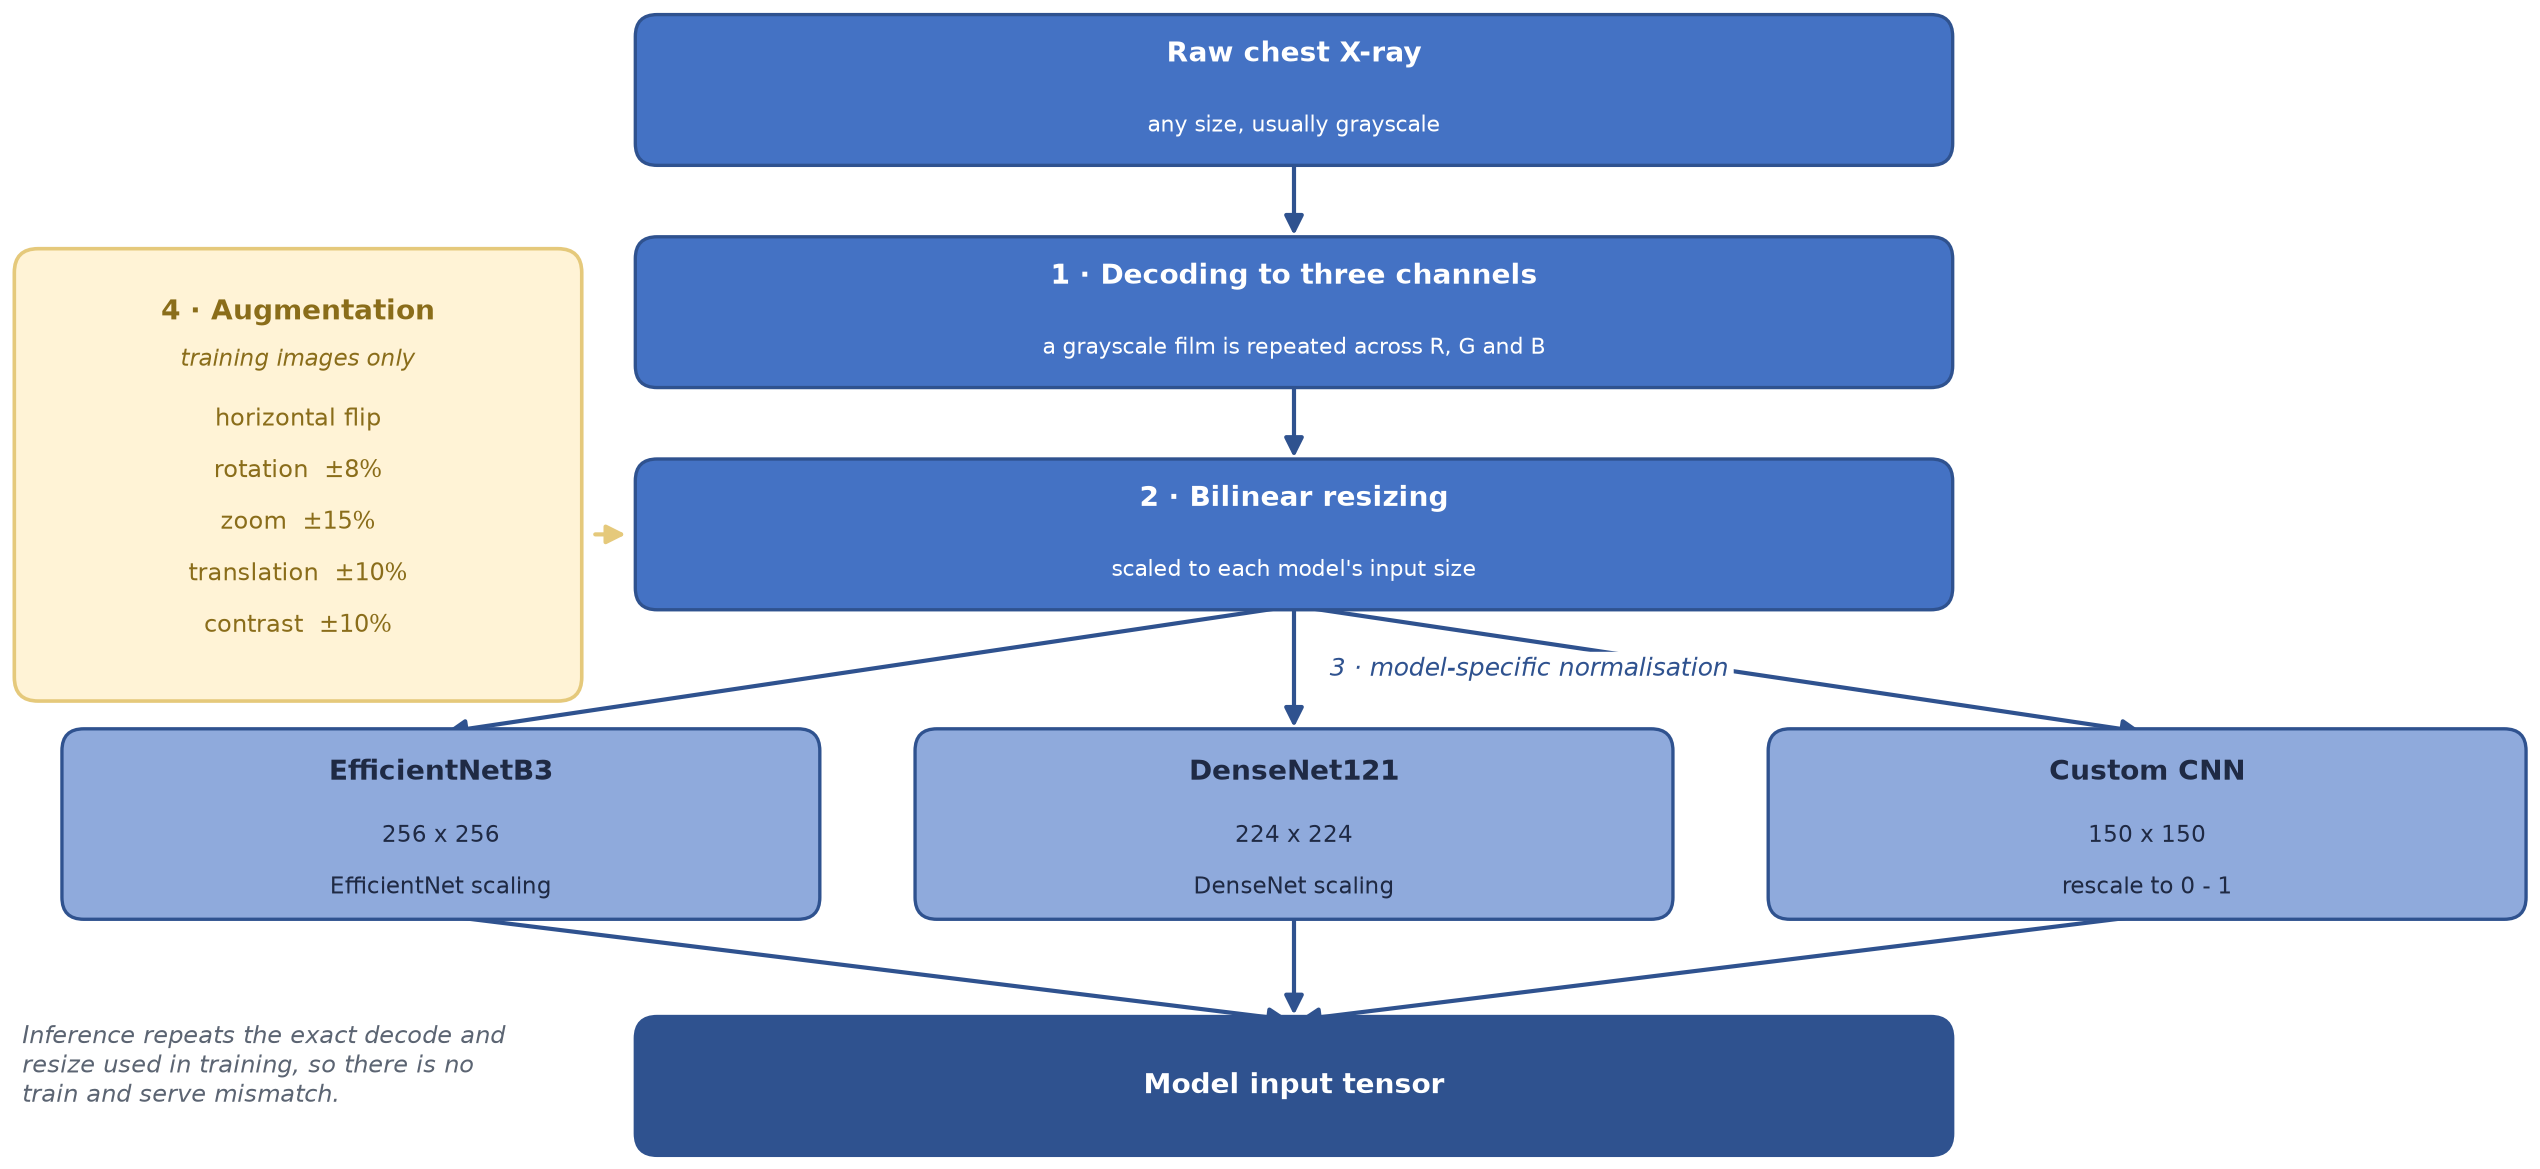
\includegraphics[width=0.95\textwidth]{images/diagrams/preprocessing_pipeline.png}
\caption{Preprocessing and augmentation pipeline with model-specific input sizes and normalisation}
\label{fig:preprocess-pipeline}
\end{figure}

\subsection{Augmentation and Class Imbalance}

All three architectures get the same geometric augmentation from the shared data pipeline: rotation, translation, zoom, and horizontal flips, each within a set range. We did not oversample the disease images. Instead, inverse-frequency class weights in the categorical cross-entropy loss make mistakes on the smaller classes cost more.

\section{Model Architectures and Shared Head}

The models are defined in \texttt{training/models.py}. Both transfer models use the same classification head, so any difference between them comes from the backbone:
\[
\text{GAP} \rightarrow \text{Dropout}(0.5) \rightarrow \text{Dense}(256,\text{ReLU}) \rightarrow \text{Dropout}(0.3) \rightarrow \text{Dense}(4,\text{softmax}).
\]
Every model ends in a softmax layer trained with categorical cross-entropy, which fixes an earlier bug where a sigmoid output was paired with that loss. None of the models start from the old single-disease weights.

\begin{figure}[H]
\centering
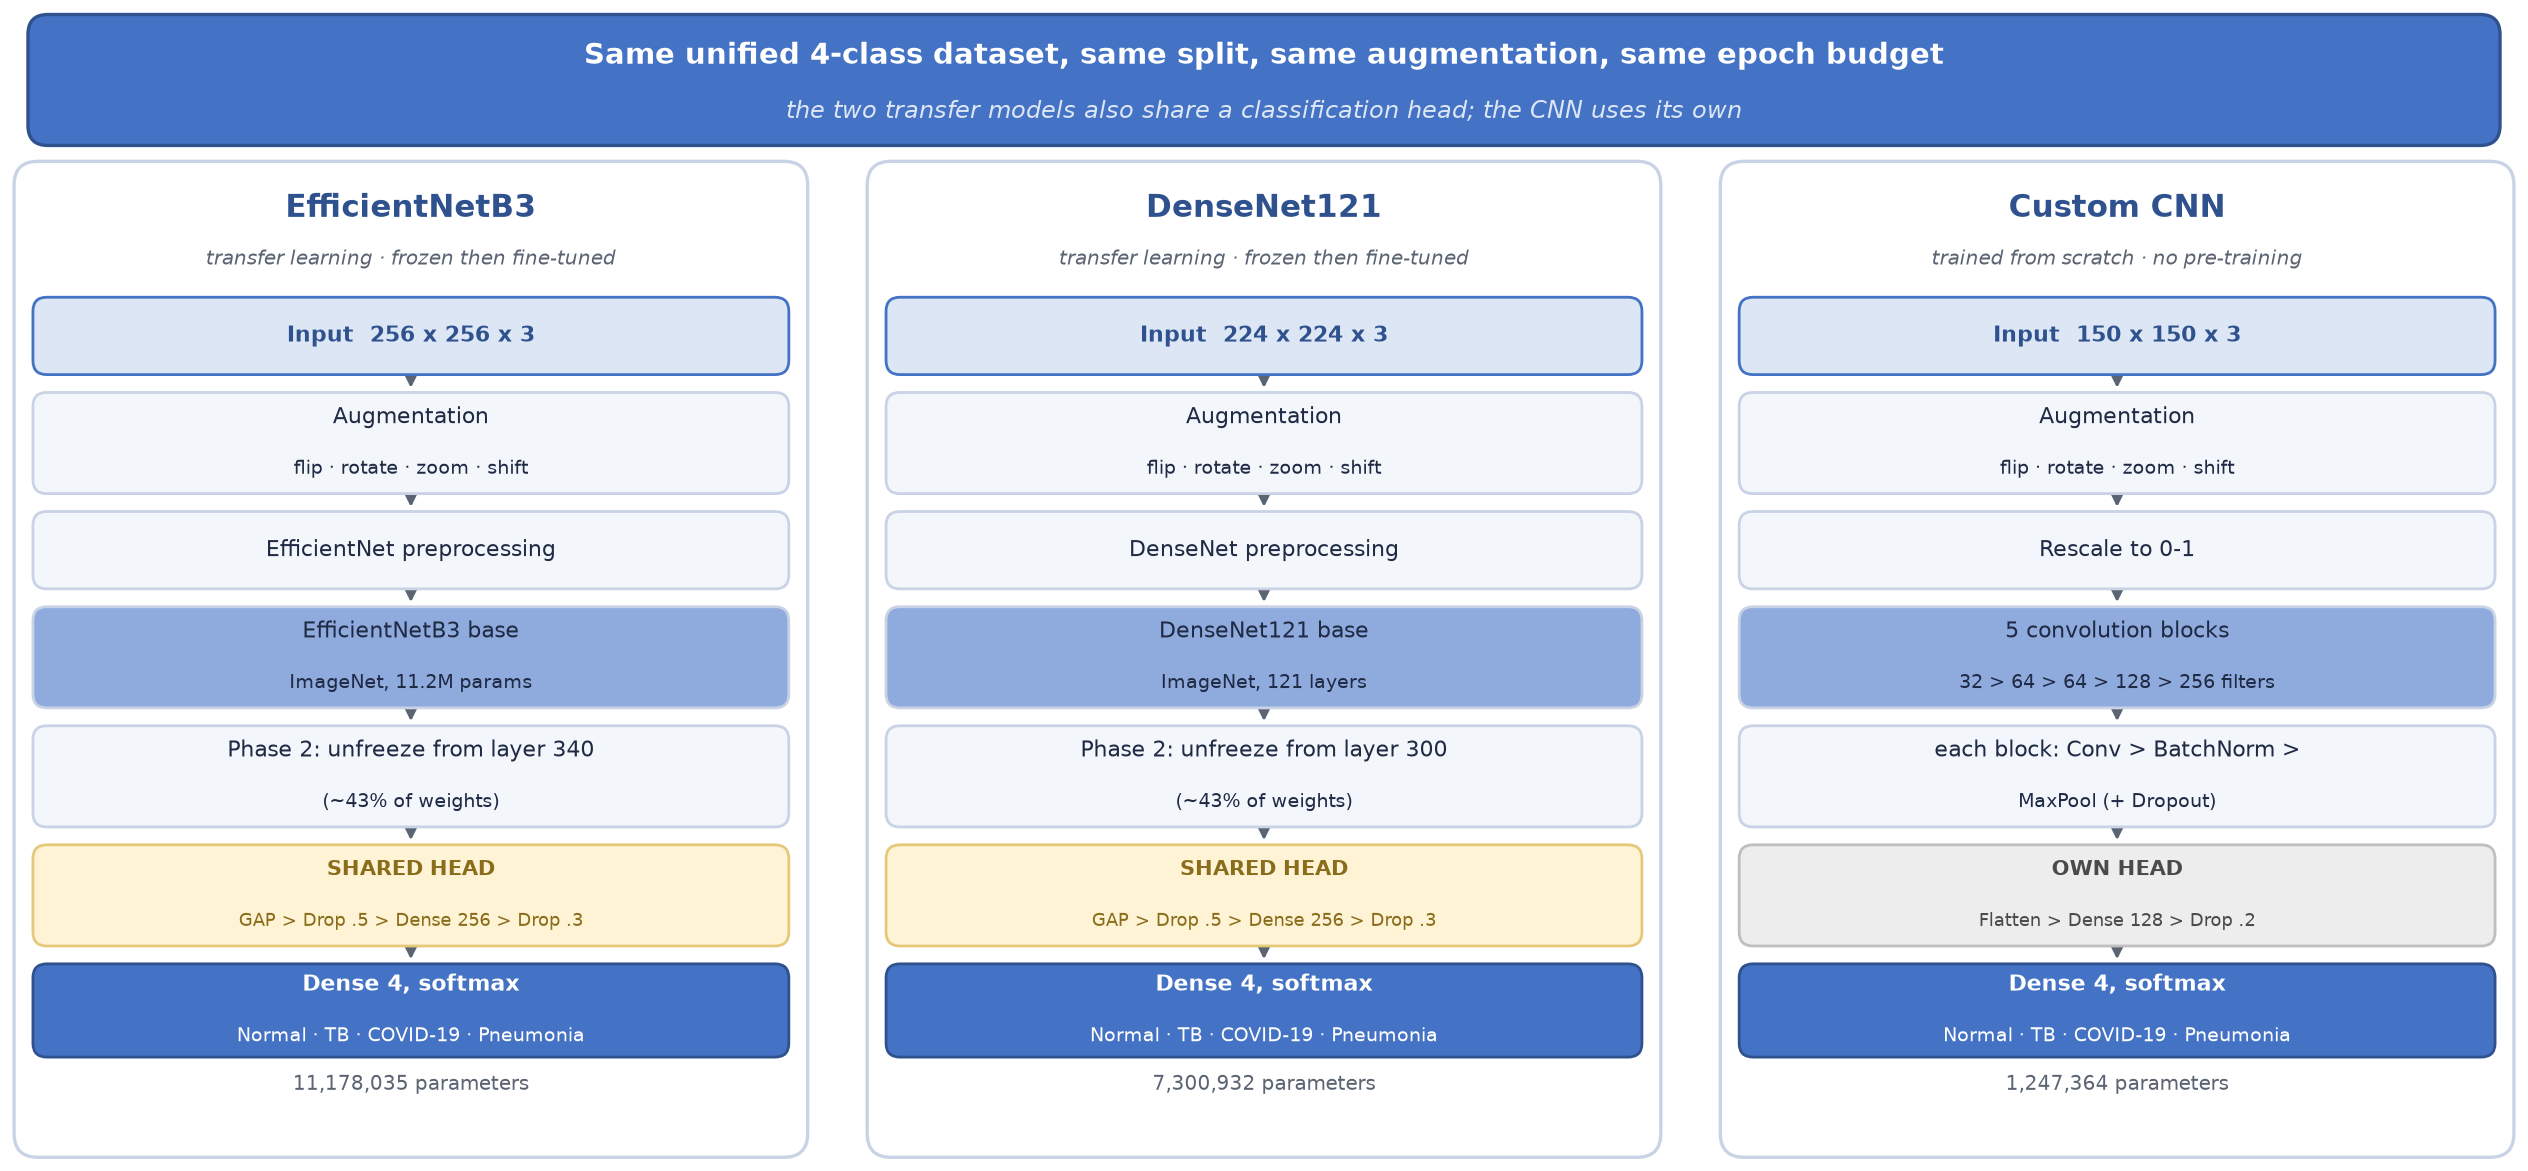
\includegraphics[width=0.95\textwidth]{images/diagrams/model_architectures.png}
\caption{Three architectures scored under a matched four-class protocol (shared head for transfer models)}
\label{fig:model-arch}
\end{figure}

EfficientNetB3 and DenseNet121 both start from ImageNet weights. In Phase~2, EfficientNetB3 is unfrozen from layer 340 onward ($\sim$42.7\% of its parameters) and DenseNet121 from layer 300 ($\sim$42.8\%), and DenseNet121's BatchNorm layers stay frozen during fine-tuning. The custom CNN is our from-scratch baseline: five convolutional blocks (filters $32\rightarrow64\rightarrow64\rightarrow128\rightarrow256$) with BatchNorm, pooling, and dropout, ending in a four-class softmax head.

\section{Training Protocol}

\begin{table}[H]
\centering
\caption{Shared training hyperparameters and controls}
\label{tab:method-hparams}
\small
\begin{tabular}{@{}P{4.5cm}P{7.5cm}@{}}
\toprule
\HeaderRow \Head{Setting} & \Head{Value} \\
\midrule
Shared seed & 1337 \\
\ZebraRow Batch size & 32 (identical across models when resources allow) \\
Phase-1 learning rate & $1\times10^{-4}$ (Adam), backbone frozen \\
\ZebraRow Phase-2 learning rate & $1\times10^{-5}$ (Adam), partial unfreeze for transfer models \\
Loss & Categorical cross-entropy with class weights \\
\ZebraRow Output & 4-way softmax \\
Test set & Never used for training or model selection \\
\ZebraRow Artefacts & \texttt{weights/*\_4class.keras}, \texttt{training/runs/*.json} \\
\bottomrule
\end{tabular}
\end{table}

\begin{figure}[H]
\centering
\begin{tikzpicture}[node distance=0.7cm]
\node[diag start, minimum width=3.2cm] (p1) {Phase 1\\Frozen backbone\\LR $1\times10^{-4}$};
\node[diag step, right=of p1, minimum width=3.4cm] (p2) {Phase 2\\Partial unfreeze $\sim$43\%\\LR $1\times10^{-5}$};
\node[diag out, right=of p2, minimum width=2.8cm] (w) {Save\\4-class .keras};

\draw[diag arrow] (p1) -- (p2);
\draw[diag arrow] (p2) -- (w);

\node[diag label, below=0.2cm of p1] {train head only};
\node[diag label, below=0.2cm of p2] {BN frozen; Adam};
\node[diag label, below=0.2cm of w] {seed 1337; class weights};
\end{tikzpicture}
\caption{Two-phase transfer-learning protocol used for EfficientNetB3 and DenseNet121}
\label{fig:train-phases}
\end{figure}

Training uses checkpointing, early stopping, and ReduceLROnPlateau callbacks. One command trains all three models: \texttt{python training/train.py --model all}.

\section{Evaluation Methodology}

The script \path{training/evaluate.py} scores every model on the held-out test split. It reports accuracy, balanced accuracy (the mean of per-class recall), per-class precision, recall, and F1, confusion matrices, a comparison across architectures, and soft-voting ensemble metrics, and writes them to \path{training/results/comparison.md}. Soft voting averages the models' probability vectors and picks the class with the highest average. Unlike a hard majority vote, it keeps track of how confident each model was.

\begin{figure}[H]
\centering
\begin{tikzpicture}[node distance=0.55cm and 0.5cm]
\node[diag step, minimum width=2.3cm] (test) {Held-out\\test set};
\node[diag model, right=of test] (m1) {EffNetB3};
\node[diag model, below=of m1] (m2) {DenseNet};
\node[diag model, below=of m2] (m3) {CNN};
\node[diag step, right=1.2cm of m2, minimum width=2.6cm] (met) {Per-class\\P / R / F1 + CM};
\node[diag out, right=of met, minimum width=2.4cm] (ens) {Soft-vote\\ensemble};
\node[diag gate, below=1.0cm of met, minimum width=2.8cm] (leak) {Leakage probe\\(source accuracy)};

\draw[diag arrow] (test.east) -- ++(0.35,0) |- (m1.west);
\draw[diag arrow] (test.east) -- ++(0.35,0) |- (m2.west);
\draw[diag arrow] (test.east) -- ++(0.35,0) |- (m3.west);
\draw[diag arrow] (m1.east) -- ++(0.4,0) |- (met.west);
\draw[diag arrow] (m2) -- (met);
\draw[diag arrow] (m3.east) -- ++(0.4,0) |- (met.west);
\draw[diag arrow] (met) -- (ens);
\draw[diag arrow] (met) -- (leak);
\end{tikzpicture}
\caption{Evaluation flow: matched test scoring, ensemble soft voting, and source-leakage probe}
\label{fig:eval-flow}
\end{figure}

The leakage probe (\texttt{training/leakage\_probe.py}) trains a classifier to predict which dataset each image came from and compares it with a majority-class baseline. Ideally it does little better than the baseline. If it could name the source almost perfectly, a model might be recognising TB or COVID-19 from how the images were acquired instead of from the disease itself. COVID-19 recall is the weakest point of the evaluation, because the class has so few test images.

\section{Application Integration Workflow}

In the application, the user uploads a PNG, JPG, or JPEG file of up to 16\,MB. The image goes through the three-stage chest X-ray gate, unless the user chooses Analyse anyway. \texttt{predict\_all()} then runs every model on it, the soft-voting ensemble combines their outputs, and the results page shows each model's probability bars, the verdict, and whether the models agree. Weight files must output four classes, and legacy \texttt{.h5} files are rejected. To reproduce the whole system, run \path{build_manifest.py}, then \path{train.py --model all}, then \path{evaluate.py}, optionally \path{leakage_probe.py}, and finally \path{Frontend/app.py} to start the application.

\section{Methodological Validity and Limitations}

The comparison is valid because the task is clearly defined, leakage is controlled, the architectures are trained the same way, the metrics include per-class recall, and deployment uses the same preprocessing as training. It has known limits. The public datasets are small, and COVID-19 recall is statistically unstable. Four-class accuracy will be lower than the old binary figures. TB and COVID-19 each come from a single source, so a model could learn source cues instead of disease (which is why we run the leakage probe). The system is not a clinical device, and Grad-CAM and multi-centre validation are left for future work.

\section{Summary}

We replaced three separate detectors with one four-class benchmark in which three architectures share the same data, splits, and training protocol, with leakage controls and ensemble deployment. Because the data and protocol are shared, differences between the models can be attributed to the architectures. The evaluation also states plainly what the datasets cannot show and that the system is not for diagnosis.
